\documentclass[conference]{IEEEtran}
\usepackage{cite, graphicx}
% *** CITATION PACKAGES ***
%
%\usepackage{cite}
% cite.sty was written by Donald Arseneau
% V1.6 and later of IEEEtran pre-defines the format of the cite.sty package
% \cite{} output to follow that of IEEE. Loading the cite package will
% result in citation numbers being automatically sorted and properly
% "compressed/ranged". e.g., [1], [9], [2], [7], [5], [6] without using
% cite.sty will become [1], [2], [5]--[7], [9] using cite.sty. cite.sty's
% \cite will automatically add leading space, if needed. Use cite.sty's
% noadjust option (cite.sty V3.8 and later) if you want to turn this off.
% cite.sty is already installed on most LaTeX systems. Be sure and use
% version 4.0 (2003-05-27) and later if using hyperref.sty. cite.sty does
% not currently provide for hyperlinked citations.
% The latest version can be obtained at:
% http://www.ctan.org/tex-archive/macros/latex/contrib/cite/
% The documentation is contained in the cite.sty file itself.

% *** GRAPHICS RELATED PACKAGES ***
%
\ifCLASSINFOpdf
  % \usepackage[pdftex]{graphicx}
  % declare the path(s) where your graphic files are
  % \graphicspath{{../pdf/}{../jpeg/}}
  % and their extensions so you won't have to specify these with
  % every instance of \includegraphics
  % \DeclareGraphicsExtensions{.pdf,.jpeg,.png}
\else
  % or other class option (dvipsone, dvipdf, if not using dvips). graphicx
  % will default to the driver specified in the system graphics.cfg if no
  % driver is specified.
  % \usepackage[dvips]{graphicx}
  % declare the path(s) where your graphic files are
  % \graphicspath{{../eps/}}
  % and their extensions so you won't have to specify these with
  % every instance of \includegraphics
  % \DeclareGraphicsExtensions{.eps}
\fi
% graphicx was written by David Carlisle and Sebastian Rahtz. It is
% required if you want graphics, photos, etc. graphicx.sty is already
% installed on most LaTeX systems. The latest version and documentation can
% be obtained at: 
% http://www.ctan.org/tex-archive/macros/latex/required/graphics/
% Another good source of documentation is "Using Imported Graphics in
% LaTeX2e" by Keith Reckdahl which can be found as epslatex.ps or
% epslatex.pdf at: http://www.ctan.org/tex-archive/info/
%
% latex, and pdflatex in dvi mode, support graphics in encapsulated
% postscript (.eps) format. pdflatex in pdf mode supports graphics
% in .pdf, .jpeg, .png and .mps (metapost) formats. Users should ensure
% that all non-photo figures use a vector format (.eps, .pdf, .mps) and
% not a bitmapped formats (.jpeg, .png). IEEE frowns on bitmapped formats
% which can result in "jaggedy"/blurry rendering of lines and letters as
% well as large increases in file sizes.
%
% You can find documentation about the pdfTeX application at:
% http://www.tug.org/applications/pdftex

% *** PDF, URL AND HYPERLINK PACKAGES ***
%
%\usepackage{url}
% url.sty was written by Donald Arseneau. It provides better support for
% handling and breaking URLs. url.sty is already installed on most LaTeX
% systems. The latest version can be obtained at:
% http://www.ctan.org/tex-archive/macros/latex/contrib/misc/
% Read the url.sty source comments for usage information. Basically,
% \url{my_url_here}.

% *** Do not adjust lengths that control margins, column widths, etc. ***
% *** Do not use packages that alter fonts (such as pslatex).         ***
% There should be no need to do such things with IEEEtran.cls V1.6 and later.
% (Unless specifically asked to do so by the journal or conference you plan
% to submit to, of course. )


% correct bad hyphenation here
\hyphenation{op-tical net-works semi-conduc-tor}


\begin{document}
%
% paper title
% can use linebreaks \\ within to get better formatting as desired
\title{NASA: Optimization of Airport Surface Planning and Scheduling}

% author names and affiliations
% use a multiple column layout for up to three different
% affiliations
%\author{\IEEEauthorblockN{Anshu Rajendra, Heron Yang, Ritwik Rajendra}
%\IEEEauthorblockA{Information Networking Institute\\
%Carnegie Mellon University\\
%anshur@andrew.cmu.edu}
%\and
%\IEEEauthorblockN{Heron Yang}
%\IEEEauthorblockA{Information Networking Institute\\
%Carnegie Mellon University\\
%heronyang@cmu.edu}
%\and
%\IEEEauthorblockN{Ritwik Rajendra}
%\IEEEauthorblockA{Information Networking Institute\\
%Carnegie Mellon University\\
%ritwikr@cmu.edu}}

% conference papers do not typically use \thanks and this command
% is locked out in conference mode. If really needed, such as for
% the acknowledgment of grants, issue a \IEEEoverridecommandlockouts
% after \documentclass

% for over three affiliations, or if they all won't fit within the width
% of the page, use this alternative format:
% 
\author{\IEEEauthorblockN{Anshu Rajendra\IEEEauthorrefmark{1},
Heron Yang\IEEEauthorrefmark{2},
Ritwik Rajendra\IEEEauthorrefmark{3},
Robert A. Morris\IEEEauthorrefmark{4},
Corina Pasareanu\IEEEauthorrefmark{5}
}
\IEEEauthorblockA{\IEEEauthorrefmark{1}\IEEEauthorrefmark{2}\IEEEauthorrefmark{3}Information Networking Institute\\
Carnegie Mellon University}
\IEEEauthorblockA{\IEEEauthorrefmark{1}anshur@andrew.cmu.edu, \IEEEauthorrefmark{2}heronyang@cmu.edu, \IEEEauthorrefmark{3}ritwikr@cmu.edu}
\IEEEauthorblockA{\IEEEauthorrefmark{4}
    Sponsor Mentor\\
    NASA Ames Research Center\\
robert.a.morris@nasa.gov}
\IEEEauthorblockA{\IEEEauthorrefmark{5}
    Advisor\\
    Carnegie Mellon University Silicon Valley\\
corina.pasareanu@west.cmu.edu}
}

% make the title area
\maketitle


\begin{abstract}
    This paper introduces planning and scheduling in the context of real world uncertainty. It demonstrates the use of probabilistic modeling to develop and implement scalable optimization algorithms to improve surface operations at large airports. As part of practicum work, we created a generic airport simulation tool (ASSET2) that is easily extensible to different scenarios and airports and improves upon the basic ASSET simulator used in this context before. We also explored different auto-scheduling methods to compare with current FCFS method. We created an uncertainty aware scheduler which produces roust schedules with simulated uncertainty. Lastly, we built a uncertainty module to model real word uncertainty and evaluate the robustness of scheduler in light of different scenarios. 
\end{abstract}
% IEEEtran.cls defaults to using nonbold math in the Abstract.
% This preserves the distinction between vectors and scalars. However,
% if the journal you are submitting to favors bold math in the abstract,
% then you can use LaTeX's standard command \boldmath at the very start
% of the abstract to achieve this. Many IEEE journals frown on math
% in the abstract anyway.

% Note that keywords are not normally used for peerreview papers.
\begin{IEEEkeywords}
    Simulation, Planning, Scheduling, Airport
\end{IEEEkeywords}

% For peer review papers, you can put extra information on the cover
% page as needed:
% \ifCLASSOPTIONpeerreview
% \begin{center} \bfseries EDICS Category: 3-BBND \end{center}
% \fi
%
% For peerreview papers, this IEEEtran command inserts a page break and
% creates the second title. It will be ignored for other modes.
\IEEEpeerreviewmaketitle

\section{Introduction}
Congestion at key airports as the area in which the traffic capacity problem is most prominent. Capacity gain requires construction of new runways and expansion of surface area for taxiing. Capacity gain means more complexity in Air Traffic Control (ATC) operations, increasing risk of human error, operator workload, and the potential for inefficiencies in operations. Capacity gain also means potentially harmful effects on the environment, such as more noise and air pollution, and higher fuel costs for taxiing aircraft. The practical difficulties of increasing capacity through airport expansion introduce the desire for enhanced airport ground movement efficiency by the intelligent use of the existing resources. The problem to be solved is a logistics problem: the coordinated movement of humans and machines to accomplish a complex task: getting arriving aircraft to gates and departing aircraft in the air. Safety and efficiency in operations are the primary goals of this work. These factors comprise the major goals of this practicum work.

Efficiency means smart planning and scheduling and also being able to use data to make smart predictions. Smart planning comprises of generating sequences of actions or events in order to achieve a goal. Smart scheduling incorporates assigning times and resources (gates, taxiways, runways) to actions in a plan. Another important concept is feasibility of the plan. A plan or schedule is feasible if it does not violate any constraints associated with the (planning or scheduling) problem to be solved. Furthermore, uncertainty can make feasible plans infeasible. For this reason it is necessary to manage uncertainty in operations. For example, if a pushback is delayed, it may not be possible to execute a planned runway ordering. A change needs to be made to a plan, for example a reordering of the runway sequence, in order to make it feasible again. The model along with these constraints describes our problem statement. We address this problem using a uncertainty-aware scheduler which has never been used in this context before. Our scheduler is able to predict the world uncertainty and incorporate it into the decision making process while building the schedule and hence produce robust schedules.

The principal contributions of this research are stated below. This paper introduces three modules that work in sync to solve the surface optimization problem at airports.

\begin{enumerate}
    \item The simulator provides a graphical representation of the airport surface, where nodes represent locations and paths represent direct paths between locations.
    \item The uncertainty-aware scheduler uses the simulator and uncertainty module to improve robustness of the system.
    \item Lastly, the uncertainty module injects random delays in our model using the Markov model to simulate point uncertainty in our system. 
\end{enumerate}

\section{Previous Work}

In this section, we provide a summary of the existing research for the ground movement problem at airports. Previous work in airport simulation has made use of ASSET simulator~\cite{morris2016planning} to represent the airport model. ASSET stands for Airport Surface Simulator and Evaluation Tool which is based on the SARDA (Spot and Runway Departure Advisor) concept. ASSET acts as a Decision Support Tool (DST) for surface management framework for scheduling, but with reduced capabilities that allows for rapid prototyping of route planning and scheduling algorithms~\cite{malik2016exact}. Furthermore, there is no concept of real world uncertainty attached to the previous model and the scheduler is hence limited to generating schedules which might not be feasible in real scenarios.

Previous work in airport scheduling makes use of two different forms of approaches. The first form has involved the development of a Mixed Integer Linear Programming (MILP) formulation, to which a commercial solver was usually applied, yielding an optimal solution. The second form of approaches has comprised of applying heuristic methods such as Genetic algorithms to reach at a optimum solution efficiency. Being a heuristic approach, GAs give no guarantee of the optimality of the solutions found. However, their success over far shorter execution times can sometimes more than compensate for this~\cite{atkin2010airport}.

Previously, three different MILP modeling approaches have been adopted to solve the airport scheduling problem. The first approach is the Exact position approach wherein a time is allocated for each aircraft to traverse each individual part of its path. The approaches of Mar ́ın~\cite{marin2006airport}, Balakrishnan and Jung~\cite{roling2008optimal} used a space-time network for this purpose. A spacial network representing the map of the airport is used as a starting point, then time is discretized and a copy of the underling spacial network is created for each time unit. These are then used to build a time expanded network. The second approach is the ordering approach wherein rather than dealing directly with timings, the algorithm first aims to decide upon the sequencing, then uses this information to schedule times for each aircraft at each node or edge. The last approach comprises of immediate predecessor/successor approach which aims at generating only the immediate predecessor and successor for each aircraft at each node/edge rather than a full sequencing. The second form of approaches i.e genetic algorithms comprise of  search methods inspired by evolutionary biology. They incorporate the ideas of natural selection, mutation and crossover~\cite{burke2005search}. GAs maintain a population of candidate solutions, have a method (called a fitness function) for evaluating solutions and apply a selection mechanism to guide the algorithm towards good solutions. The correct encoding of the problem can be key for the successful application of a GA, as can be the choice of appropriate mutation and crossover operators for the selected problem encoding. As for the MILP approaches, the GAs consider either the absolute timing or the relative sequencing of the ground movement. Lastly, to the best of our knowledge, there has been no previous research in modeling uncertainty at airports and developing a scheduler that takes into account the real world uncertainty to generate schedules.

\section{Architecture}

By following the architecture of ASSET designed by NASA, we built ASSET2 which shares a similar architecture but slightly different design goals. We include few missing components in ASSET including the uncertainty module, graphic monitor integration, and supports in multiple airport data. ASSET2 is designed to enable us to learn the performance of different kind of scheduler with different control variables including the amount of uncertainty, the scale of tightness, the reschedule time, etc.

The system is divided into three parts and followings are the design goals of each part.

\paragraph{Simulation}

\begin{enumerate}
    \item Works for multiple airports sharing the same link-node model
    \item Works with an external scheduler in runtime, and be able to show performances
    \item Be extensible for adding new constraints, features in the future
\end{enumerate}

\paragraph{Scheduler}

\begin{enumerate}
    \item Repeatedly generates schedules for aircrafts that enter the airport during the day
    \item Ensures that the schedules generated are free of conflicts in the absence of uncertainty
    \item Uses the simulation to predict possible airport state in the future, and relax tightness at possible bottlenecks
\end{enumerate}

\paragraph{Uncertainty Module}

\begin{enumerate}
    \item Enables users to manipulate different factors for creating uncertainties in the system
    \item Integrates with external scheduler and simulator in runtime and be controlled by the user to inject randomness
    \item Takes terminal uncertainty at gates and runways into account
\end{enumerate}

\subsection{Flow}

\begin{figure}
\centering
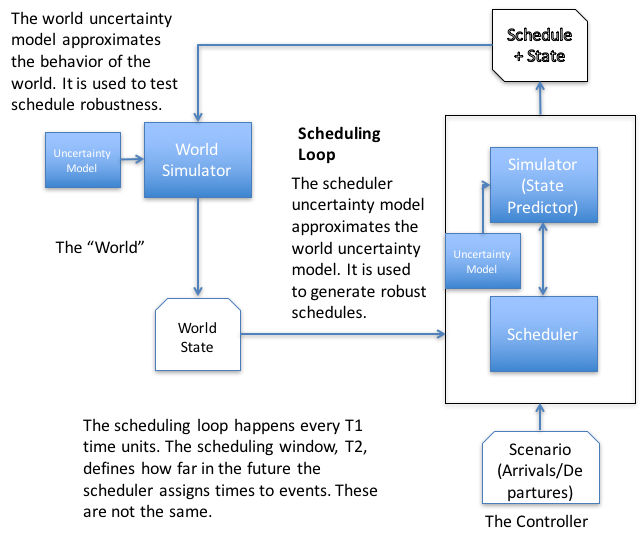
\includegraphics[width=2.8in]{flow}
\caption{Scheduling Flow in Simulation\label{flow}}
\end{figure}

Figure \ref{flow} describes the design of different states. Simulator owns a state of the airport that we currently simulating, which we call it World State. World State contains uncertainty that the scheduler will never be able to fully predicts, and it's used to create chaos just like what we usually see in the real world.

On the other hand, the scheduler is able to consult the simulator to simulate future states with specific amount of uncertainties. But, the uncertainties here are not the same one as the one actually be used by the simulation because the schedule should not be able to know the real world uncertainty. By running multiple predictions while scheduling, the scheduler will be able to provide a better schedule for the simulation. Finally, the simulator will analysis the performance of the scheduler in the end by looking at metrics we are interested while there's some different amount of uncertainties.

\section{Implementation}

\begin{figure*}[!t]
\centering
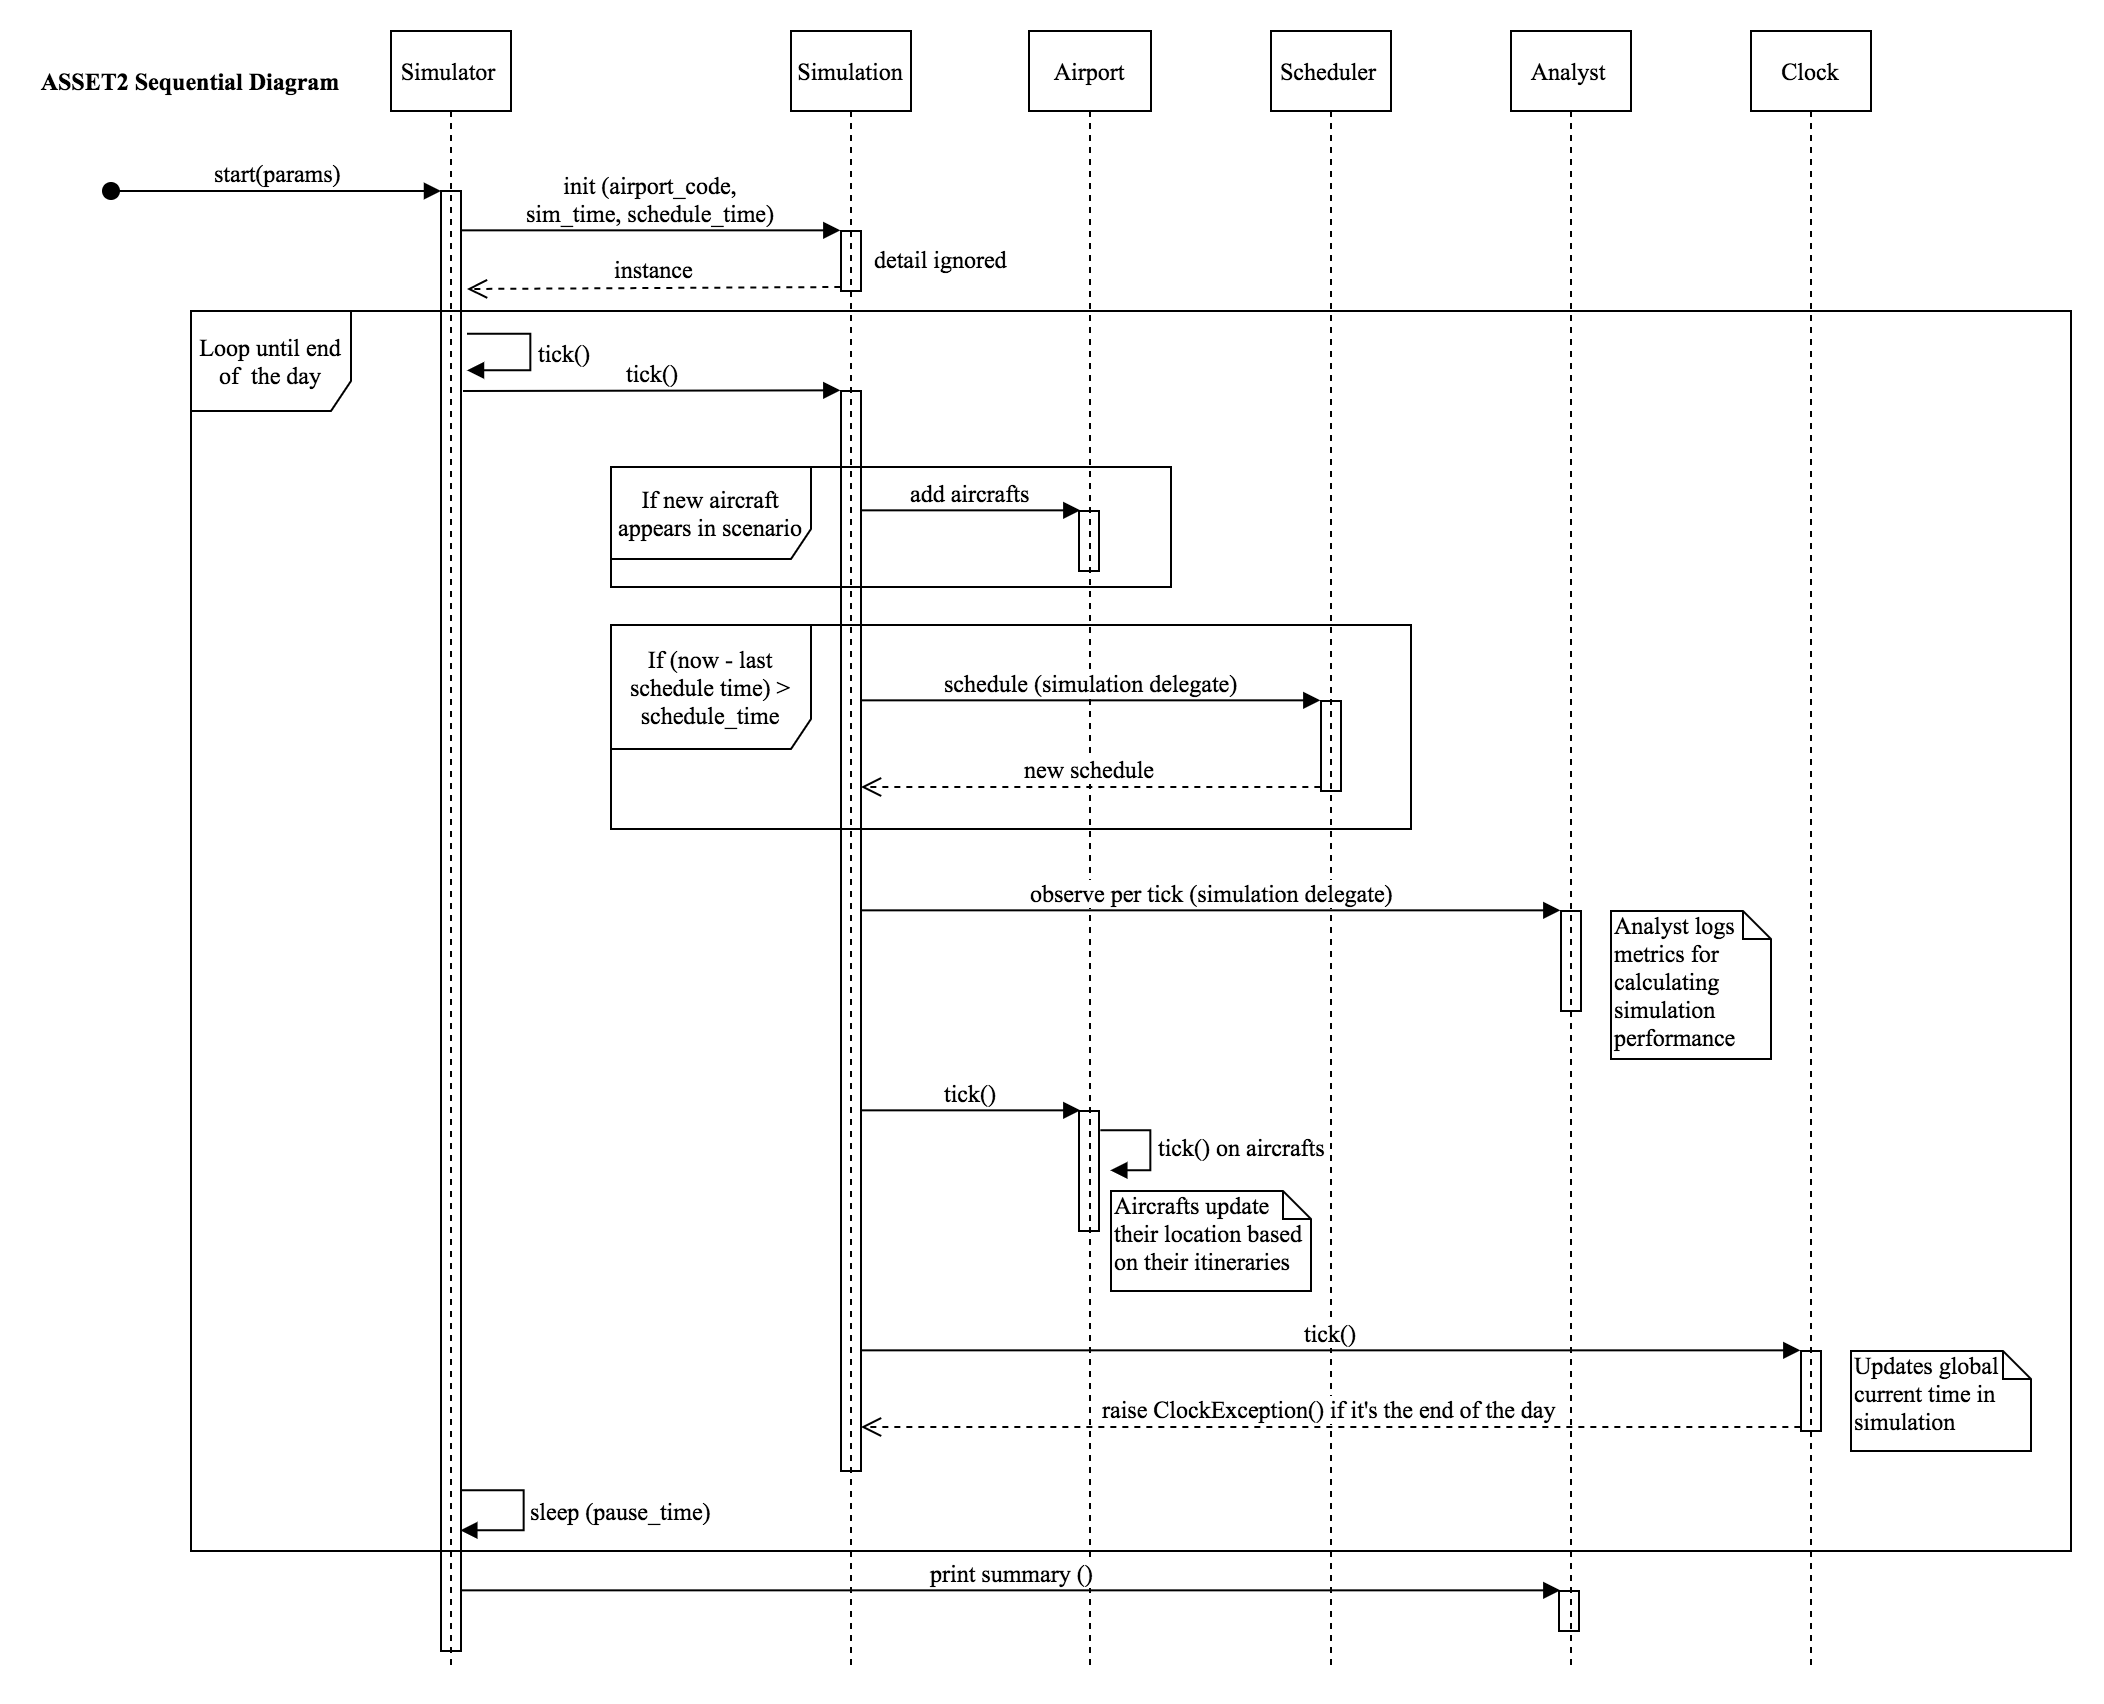
\includegraphics[width=\textwidth,height=\textheight,keepaspectratio]{seq}
\caption{Sequential diagram of the whole system for simulating airport surface movements within a day\label{flow}}
\end{figure*}

First, the user initializes the simulator by passing control variables including the `reschedule time`, `the amount of uncertainty`, `scheduler tightness`, `simulated time per tick`, `real pause time per tick`, etc.

Second, the simulator starts to `tick` each components periodically, and each component moves to state in the future when it's be ticked. While `ticking` the simulation, the simulation first `ticks` all the aircrafts on the airport so they will either move to next node or stay at the original node based on the schedule assigned by the scheduler previously. Then, the simulation will add new aircrafts into the airport based on the scenario or remove aircrafts from the airport if any of them had arrived the runway. Last, it may asks the scheduler for a new schedule and distribute the schedule onto each aircraft. In each tick, the analyst object stores all the metrics that we are interested in and print out a summary in the end of the simulation.

Third, the clock object is tracking the current simulated time, and it will force the simulation to stop if we had reached the end of a day. The simulation asks the analyst to print out a summary of what it observed over the simulated day.


\subsection{Simulation}

\paragraph{Data Source}

The simulation works with different airports as long as the data is loaded under $data/<AIRPORT\_CODE>/build/$ and follows the file structures we defined. Examples can be found in $data/sfo/build/$. The files read by the simulation include airport meta data, gate data, spot position data, pushback way data, taxiway data, runway data and scenario data.

Currently, we have two airport data ready and be loaded in our repo, San Francisco Airport and Simple Airport. San Francisco Airport is parsed from OpenStreetData and Google Map data, and Simple Airport is drawn by ourselves for debugging.

\paragraph{Link Node Model}

All surface components are built from nodes or links, where links are composed by nodes. Node represents a geo point, and could be inherited by Gate, Spot Position, etc. Link represents a sequence of nodes and could be inherited by Taxiway, Runway, etc.

\paragraph{Routing}
Shortest routes between two nodes (including the two end nodes of a link) are calculated before simulation starts. The steps of building all route pairs are:

\begin{enumerate}
    \item links two nodes with distance smaller than 30ft (we assume these 2 nodes are the same spot)
    \item fills in the distance of the two end nodes
    \item run Floyd–Warshall algorithm to get all shortest path
\end{enumerate}

\paragraph{Scenario}

Scenario represents all flights information within a day. For each flight, it includes the expected departure or arrival time, the gate and runway used, and the airport information. The scenarios is currently been randomly generated as we haven't be able to retrieve a real data yet.

\subsection{Uncertainty Module}

The purpose of uncertainty module is to inject randomness into our simulation so that we make robust and realistic schedules. Uncertainty with airport surface operations comes from three sources: human decision-making, mechanical problems, and changes to the environment. A passenger on a departing flight might take too long finding an overhead bin for his bag. This might delay the pushback time for his flight. Mechanical problems to the aircraft or towing vehicles might delay or cancel a flight. Changes to weather conditions (an afternoon summer thunderstorm) typically delay all incoming and outgoing flights. Uncertainty can make feasible plans infeasible. For this reason it is necessary to manage uncertainty in operations. For example, if a pushback is delayed, it may not be possible to execute a planned runway ordering. A change needs to be made to a plan, for example a reordering of the runway sequence, in order to make it feasible again. This module injects uncertainty at two points into the model.

\paragraph{Runtime Uncertainty}

This is the actual uncertainty injected in the simulation mimicking the real world. The scheduler is unaware of the actual uncertainty in the simulation of real world and only has an idea of random range of uncertainty applied in the world. Thus the uncertainty module at this time acts as an evaluator for the performance of the scheduler and helps us to segregate more robust schedules than the others. Our system also incorporates prior belief of world uncertainty of the user using a control parameter which is then used to determine point or terminal uncertainty.

\paragraph{Simulated Uncertainty}

The uncertainty module also provides an interface to the scheduler to run simulation with uncertainty during the schedule making process to help make robust schedules. At this point, the uncertainty module acts as an advisory to the scheduler to help determine the effect of various amounts of uncertainty on the simulation and adjust the parameters of the model accordingly. Note that the uncertainty used here is independent of the real world uncertainty and hence the scheduler can only approximate world uncertainty at this time.

\subsection{Scenario}

This section provides an overview of the various points in the simulation model where we can inject uncertainty to mimic the real world scenario. Below we list out the various points and the type of uncertainty model which can be applied to each:

\paragraph{Aircraft speed} The speed of the aircraft can be expected to differ around its expected value with some variance. (Gaussian uncertainty)

\paragraph{Time uncertainty} All times in the scenario i.e arrival and departure time can be affected with gaussian uncertainty around expected value.

\paragraph{Location} Unlike speed and time which can be changed in a continuous range, location in our model can only hold certain discrete nodes and for this we can model the uncertainty as a binary parameter i.e either the vehicle changes node location with 80% probability or waits with 20% probability to mimic a scenario with 20% uncertainty.
\paragraph{Pilot decision} This could mean pilot decision to wait at a certain point which could affect flights before and after it. In any case, this can be modeled as point uncertainty or binary parameter which would mimic if the pilot did move the vehicle or not.
\paragraph{Uncertainty at terminal nodes} Distinction between appear time and actual appear time for scheduler as terminal nodes are more prone to uncertainty.

\subsection{Other Scenarios}
We could also make certain scenarios to combine many of these factors and uncertainties together which the simulator can use. Possible scenarios include:

\paragraph{Bad weather/Storm/Fog} Aircraft speed will be reduced and the uncertainty in pilot decisions and time would be increased due to bad visibility.

\paragraph{Construction/Repair} Certain random edges will not be available with total uncertainty.

\subsection{Overview of Approaches}

We implemented two approaches to uncertainty in our system. Firstly we wanted to account for nodal uncertainty which is based on markov model randomness and also wanted to inject gaussian uncertainty at different points in the module.

\paragraph{Point/Position Uncertainty} The first is position uncertainty that is derived from markov random process. The scheduler assigns routes to every aircraft in the schedule. However, in the real world the schedules are generally not followed as is due to bad weather, construction or any other random event. This module thus mimics uncertainty using the approach that there is some probability (p) to either actually move to the next node or be stranded on the current node with remaining probability (1-p). This uncertainty becomes even more pronounced at terminal nodes. By terminal nodes we mean nodes (specifically gate, taxiway enter and runway entrance nodes) at which aircraft enter and leave the surface scheduling system. Things get slightly more complex at these nodes than at internal nodes. One kind of uncertainty involves when an aircraft `actually' enters the scheduling system. The arrival flight could enter the system at 510 rather than 500, or the departure flight could be ready to depart from the gate at time 704 rather than 700. Note that `delay in ready to depart' is not the same as `delay in departure' Delay in departure is when the scheduler says `pushback' but the aircraft does not, whereas `delay in ready to depart' means that it is not ready to pushback. Another kind of uncertainty involves when an aircraft `actually' leaves the scheduling system. Here we assume there is an asymmetry here between terminal nodes for gates and terminal nodes for runways. To account for terminal uncertainty, we inject twice the randomness in delays at these points.


\paragraph{Gaussian uncertainty} In a previous approach, we used normal distribution to model uncertainty at various places in our simulator. The basic idea is that the uncertainty can be thought of as variance around the mean for a gaussian distribution and hence the problem reduces to finding the ideal variance to model uncertainty using different factors. Not only do we need to know the factors that should account the variance/uncertainty but also their relation to uncertainty. For instance, frequency of scheduling for the simulator has an inverse relation to uncertainty i.e more the frequency, lesser the model uncertainty. This module is extensible for adding new factors for uncertainty later. Note that we already have the perfect scenario values in our cases which should be the expected mean in the gaussian distribution. To calculate the variance, we take the user provided factors and for each factor either take the value directly (DIRECT) or invert it (INVERSE) and take the sum of these values as the uncertainty. Future approaches will try learning weights of this factors to determine the optimum combination of factors for calculating variance.

\section{Scheduler}

A route can be viewed as a sequence of edges of a node-link graph (equivalently, a set of nodes on the graph). In our version of the problem, the routes of all the aircraft are pre-assigned. Given a gate (for departures) or arrival runway (for arrivals), there is a single route the aircraft always takes (This single route is the shortest-time route). Knowing the edges (or nodes) that the aircraft will traverse for each flight, then the problem becomes a scheduling problem: assign times to each of the nodes or edges. At the other extreme, suppose that there are no constraints on the route than any aircraft may take. Then the solution requires finding both the route and the times for the route. This version of the problem combines path planning with scheduling. In between these extremes there are problems in which there are constraints on what routes are permissible, and the route chosen must satisfy these constraints. 

Route planning and scheduling is an optimization problem. In an optimization problems you're trying to achieve (maximizing or minimizing) some objective. Total taxi time (including delays during taxiing) is an example of an objective to minimize. In our implementation, we aim to  minimize the makespan, which is the total time it takes to process all the flights. It's possible to combine objectives into a multi-objective problem, where weights are assigned to the different objectives.

\subsection{Conflict Resolution}

As we've seen, a model of the airport surface planning problem usually starts with a graphical representation of the airport surface, where nodes represent locations and paths represent direct paths between locations. Time is not represented in this spatial model, so to do scheduling, time must be added. The simplest way to imagine the effect of adding time is to imagine making copies of the graph for a set of discrete moments in time, showing the evolution of surface flow. So instead of a route consisting of a sequence of edges, we know have a route consisting of a sequence of pairs <(e, t)> of edges and times. We define a conflict as a state where two or more aircrafts occupy the same node at the same point of time, i.e., two flight schedules contain the same <e,t> pair. The aim of the scheduler is to generate a schedule that is free of conflicts in the absence of uncertainty, and also robust to such conflicts in the presence of uncertainty as well. In our implementation, we handled conflicts by delaying one of the conflicting flights until the flight occupying the node leaves the space.

\subsection{Tightness and Replanning}
An important feature of a schedule is its tightness. Tightness measures the overall spacing between aircrafts. A tight schedule is one where the aircraft don't have a lot of space between them. Tightness is related to robustness because if there is unexpected delay for one aircraft, the overall effect is delay everywhere else in the schedule. Having a measure of tightness enables us to make intelligent decisions about how often we need to reschedule, given the chance of uncertainty. In our implementation, schedule tightness as the minimum of the node tightness for all the nodes, i.e., then a schedule is as tight as its tightest node.
We can control the effects of unexpected delays on tight schedules in two ways: by re-planning more often or by imposing tightness constraints during scheduling. An example of a tightness constraint is: no schedule should have a tightness less than 3 minutes. But the more optimal approach is to tie tightness to the the amount of re-planning that is done. If the scheduler generates a schedule that is `loose' then we expect unexpected delays to have no effect on the ability of the schedule to be executed without conflict. As a result, there is no need to reschedule often. Conversely, if a tight schedule is generated, then the world state needs to be monitored for unexpected delays to avoid conflict.


\section{Experiments}

For evaluating our modules, we ran two different sects of experiments. 

\begin{enumerate}
	\item The first experiment compared the effect of schedule tightness(defined later) with number of conflicts generated through a single run for varying amounts of uncertainty. 
	\item The second experiment compared the effect of uncertainty on scheduler replanning or in other words, how much the scheduler has to replan to mitigate the effect of uncertainty.
\end{enumerate}

We wanted to test both deterministic and nondeterministic scheduling i.e effect on world with and without uncertainty. For us, uncertainty takes the form of delays. Specifically, an aircraft is expected to leave a node at a given time, and it does not. Our uncertainty model on the simulation side (i.e. `in the world' allows us to inject delays randomly into the simulation. Furthermore, schedules can be compared with respect to the property of tightness. We defined the tightness of a node of graph in a schedule in terms of the minimum time difference between consecutive visits to the node by aircraft; and the schedule tightness is the average (or minimum) node tightness over all nodes in the graph.

In these tests we were interested in observing the ability of a schedule to be robust to conflicts during schedule execution. We know that although a schedule might be conflict-free, there may be conditions in the world that cause conflicts while the schedule is run (let's call these run-time conflicts). We want to design a scheduler so that run-time conflicts never happen. Possible approaches to mitigate the effect of uncertainty at scheduling side are as follows:

\begin{enumerate}
	\item Predict possible conflicts during scheduling (i.e. remove determinism from the scheduler). A simple way to do this would be to control the tightness of the schedule. We're saying, in effect: we expect delays during run time, so we will systematically inject delays into the schedule in anticipation of delays in the world. Unless we're lucky, this approach will lead to sub-optimal schedules with respect of minimizing delays.
	\item The other thing we can do is re-plan. This can be viewed as a sort of re-calibration: the world takes our schedule and moves it `off course' through delays. By re-planning we bring the schedule back in line with the world before run-time conflicts happen.
\end{enumerate}

To set up the experiment we needed to

\begin{enumerate}
	\item generate many schedules that differ in tightness: wrote shell scripts to carry out this task.
	\item have a procedure for detecting run-time conflicts: the simulator detected run-time conflicts
	\item have a control parameter that allows for changing the amount of uncertainty during simulation: defined a control parameter “uc” that defines the percentage of uncertainty in the run
	\item have a re-planning capability and a parameter that controls the amount of re-planning performed: The scheduler carries out replanning, and the parameter “tr” defined how often rescheduling was done. 
	\item have a way to collect statistics counting the number of conflicts that occur, for schedules of varying tightness and for varying degrees of uncertainty: The code includes a  script that collected the relevant statistics after every run. 
\end{enumerate}


\subsection{Experiment 1}

In this test the goal is to measure the effects of schedule tightness on the amount of run-time conflicts, for varying degrees of uncertainty. With no uncertainty, there are never any conflicts, no matter how tight or loose the schedule is. When you inject uncertainty, you expect a curve that peaks at the tightest schedules (tightness = 1) and goes down with less tight schedules. With more uncertainty, the curve starts higher and degrades to 0 more slowly with less tightness.

\begin{figure}[!t]
\centering
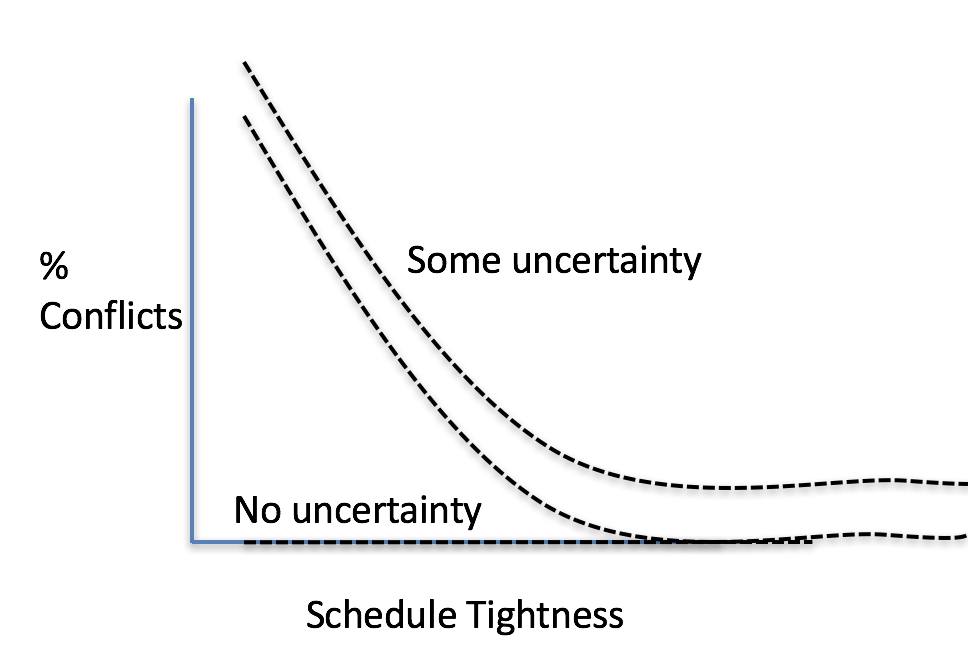
\includegraphics[width=2.8in]{exp1-expected}
\caption{Expected schedule tightness, conflicts, and uncertainty\label{exp1-expected}}
\end{figure}

The actual results were different, in the sense that although relaxing the tightness constraint initially results in decreasing conflicts, this only occurs upto a point, following which the number of conflicts again starts increasing. This is because large tightness values resulted aircrafts being delayed too much, and a pile-up occurred further forward in time between the delayed aircrafts and the newly arriving ones. 

We also plotted the results of taxi delay vs tightness for varying values of uncertainty, which showed that the taxi time time sharply increases with increasing values of tightness, with the behavior being similar to an exponential curve.

\begin{figure}[!t]
\centering
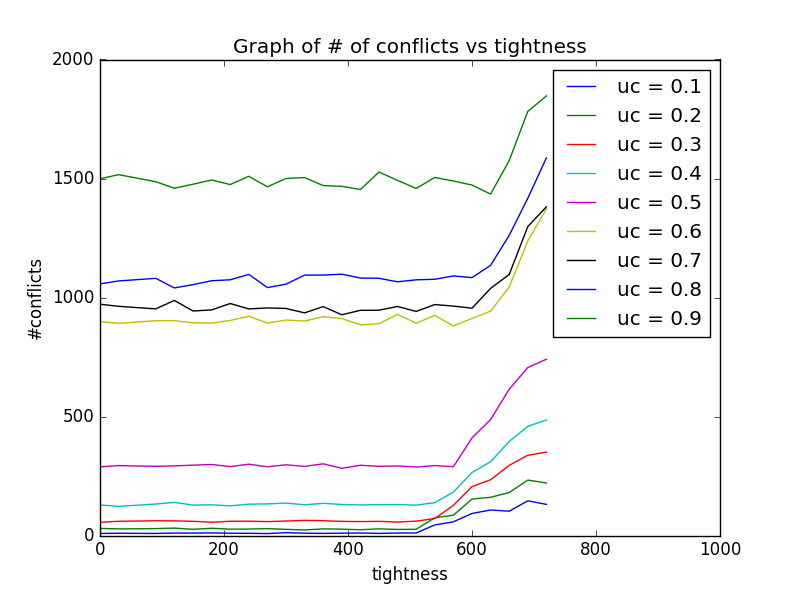
\includegraphics[width=2.8in]{exp1-g1}
\caption{Graph of schedule tightness, conflicts, and uncertainty\label{exp1-g1}}
\end{figure}

\begin{figure}[!t]
\centering
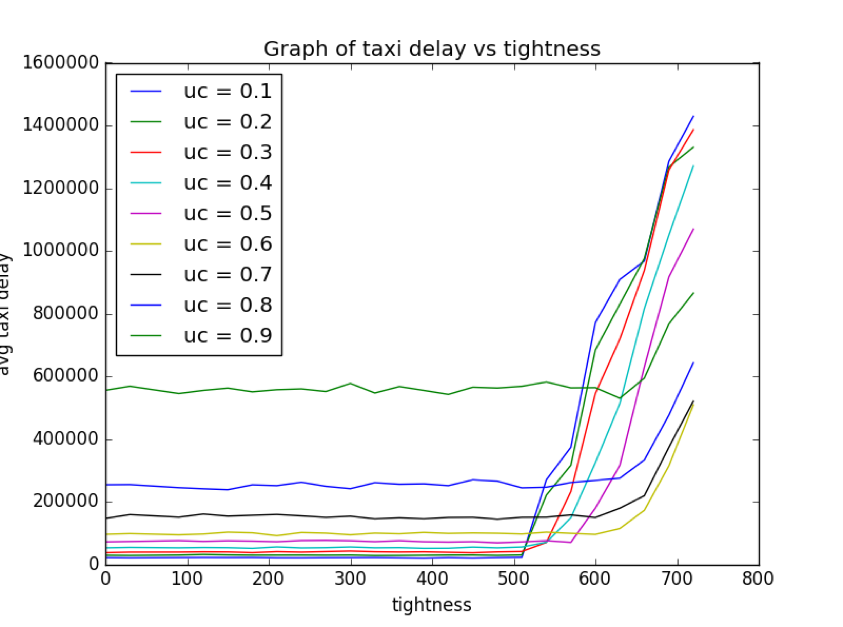
\includegraphics[width=2.8in]{exp1-g2}
\caption{Graph of schedule tightness, taxi delays, and uncertainty\label{exp1-g2}}
\end{figure}

\subsection{Experiment 2}

In this test, we fix the level of tightness and measure the effect of different levels of re-planning on the amount of run-time conflicts. We expect that at some level of re-planning, say every 5 seconds, there are never any conflict, no matter what reasonable level of uncertainty is imposed. (Of course, we could impose a `herding cats' level of uncertainty that would make it impossible to schedule anything, but this is not reasonable). In general we expect that the more re-planning we do, the more uncertainty the schedule can tolerate without run-time conflict. The results obtained confirm this hypothesis.

\begin{figure}[!t]
\centering
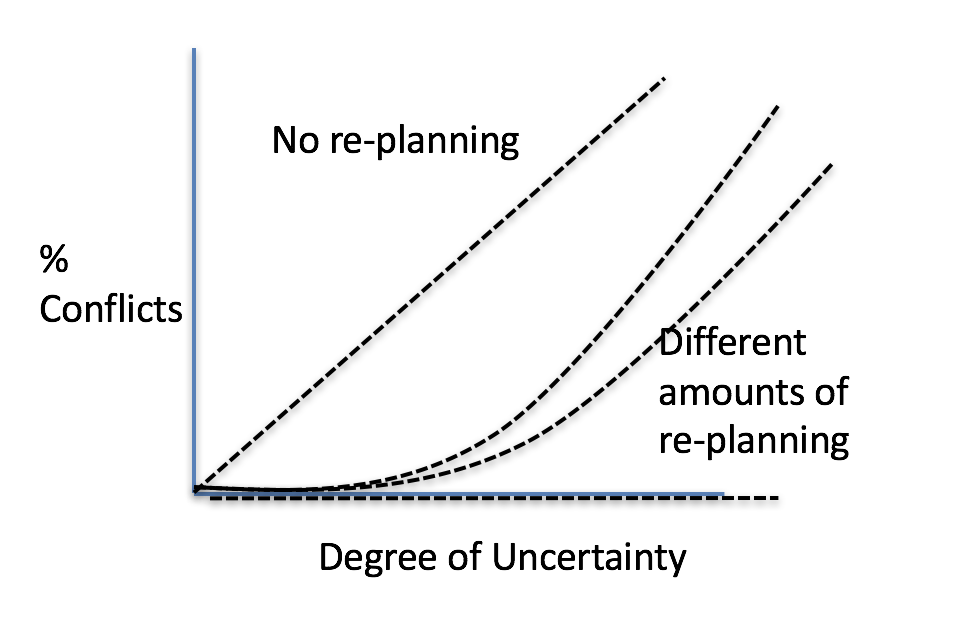
\includegraphics[width=2.8in]{exp2-expected}
\caption{Expected schedule tightness, conflicts, and uncertainty\label{exp2-expected}}
\end{figure}

\begin{figure}[!t]
\centering
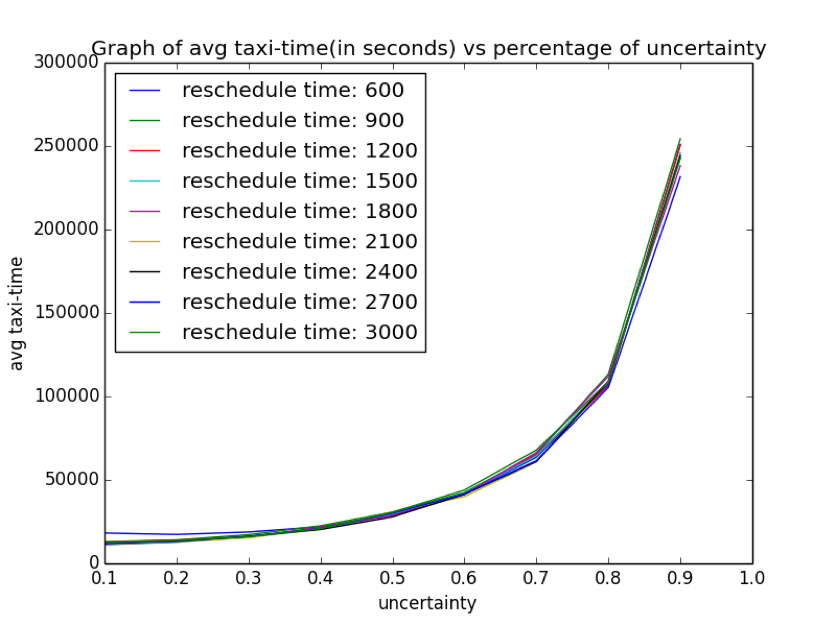
\includegraphics[width=2.8in]{exp2-g1}
\caption{Graph of average taxi-time (in seconds) v.s. percentage of uncertainty\label{exp2-g1}}
\end{figure}

\begin{figure}[!t]
\centering
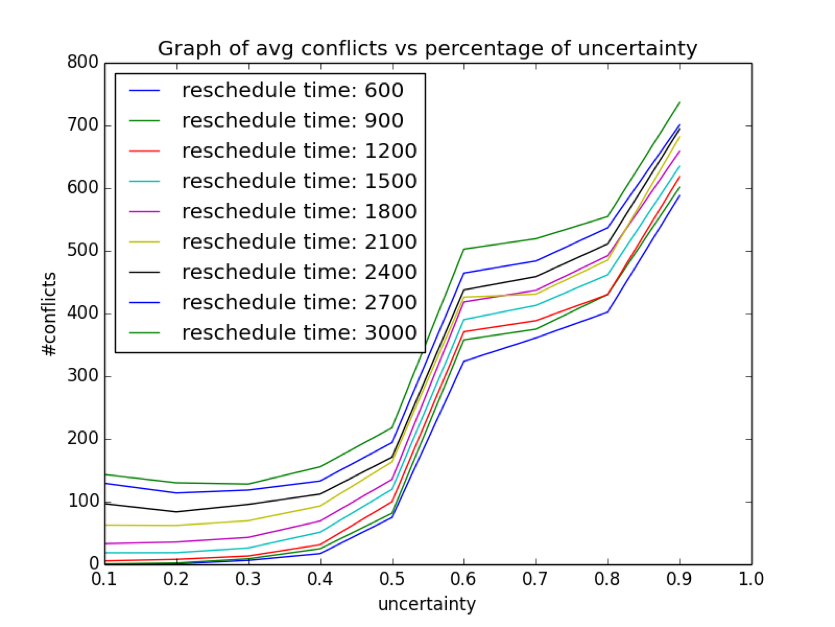
\includegraphics[width=2.8in]{exp2-g2}
\caption{Graph of average conflicts v.s. percentage of uncertainty\label{exp2-g2}}
\end{figure}

\section{Conclusion}

In this project, we've successfully built a system, ASSET2, to simulate surface movements of an airport using different scheduling algorithm with different control variables and uncertainties. The system is composed by three main modules: simulator, scheduler, and uncertainty module. Simulator is in charge of maintaining the airport state and coordinates every components in the system. Scheduler is be triggered by the simulator and offers the best schedule based on a given airport state. Uncertainty module is injected in the simulation and will create chaos for users to obverse the performance of the scheduler under uncertainty.

We ran two experiments using ASSET2 to see if we can plot the figures that we expected. In the first experiment, we measure the effects of schedule tightness on the amount of run-time conflicts for varying degrees of uncertainty. We found that the result is different because large tightness values resulted aircrafts being delayed too much. In the second experiment, we fix the level of tightness and measure the effect of different levels of re-planning on the amount of run-time conflicts, and we found the result confirm our hypothesis.

\section{Future Work}

First, there are some missing metrics that we would like to measure and run experiments on it including the maxspan and the total delay time. The maxspan is defined as the time duration between the time of the first flight arrived and the time of the last flight been removed. And, the total delay time is the time difference between the expected departure/arrival time and the real departure/arrival time. These two values should be minimized and be seem as objectives while designing the scheduler.

Second, we planned to run more tests on relatively larger airports. Currently, the experiments were done using the Simple Airport. We are looking for a more completed airport surface data for us to test our system with more realistic data.

Last, We are expecting to find out a trade-off point between robustness and performance while setting the control variables of an airport. That is, a less tight schedule usually brings less conflicts while a tighter schedule brings higher performance. A graph that shows the intersection of having maximum robustness and performance in the same time is expected in the future work.

% needed in second column of first page if using \IEEEpubid
%\IEEEpubidadjcol

% An example of a floating figure using the graphicx package.
% Note that \label must occur AFTER (or within) \caption.
% For figures, \caption should occur after the \includegraphics.
% Note that IEEEtran v1.7 and later has special internal code that
% is designed to preserve the operation of \label within \caption
% even when the captionsoff option is in effect. However, because
% of issues like this, it may be the safest practice to put all your
% \label just after \caption rather than within \caption{}.
%
% Reminder: the "draftcls" or "draftclsnofoot", not "draft", class
% option should be used if it is desired that the figures are to be
% displayed while in draft mode.
%
%\begin{figure}[!t]
%\centering
%\includegraphics[width=2.5in]{myfigure}
% where an .eps filename suffix will be assumed under latex, 
% and a .pdf suffix will be assumed for pdflatex; or what has been declared
% via \DeclareGraphicsExtensions.
%\caption{Simulation Results}
%\label{fig_sim}
%\end{figure}

% Note that IEEE typically puts floats only at the top, even when this
% results in a large percentage of a column being occupied by floats.


% An example of a double column floating figure using two subfigures.
% (The subfig.sty package must be loaded for this to work.)
% The subfigure \label commands are set within each subfloat command, the
% \label for the overall figure must come after \caption.
% \hfil must be used as a separator to get equal spacing.
% The subfigure.sty package works much the same way, except \subfigure is
% used instead of \subfloat.
%
%\begin{figure*}[!t]
%\centerline{\subfloat[Case I]\includegraphics[width=2.5in]{subfigcase1}%
%\label{fig_first_case}}
%\hfil
%\subfloat[Case II]{\includegraphics[width=2.5in]{subfigcase2}%
%\label{fig_second_case}}}
%\caption{Simulation results}
%\label{fig_sim}
%\end{figure*}
%
% Note that often IEEE papers with subfigures do not employ subfigure
% captions (using the optional argument to \subfloat), but instead will
% reference/describe all of them (a), (b), etc., within the main caption.


% An example of a floating table. Note that, for IEEE style tables, the 
% \caption command should come BEFORE the table. Table text will default to
% \footnotesize as IEEE normally uses this smaller font for tables.
% The \label must come after \caption as always.
%
%\begin{table}[!t]
%% increase table row spacing, adjust to taste
%\renewcommand{\arraystretch}{1.3}
% if using array.sty, it might be a good idea to tweak the value of
% \extrarowheight as needed to properly center the text within the cells
%\caption{An Example of a Table}
%\label{table_example}
%\centering
%% Some packages, such as MDW tools, offer better commands for making tables
%% than the plain LaTeX2e tabular which is used here.
%\begin{tabular}{|c||c|}
%\hline
%One & Two\\
%\hline
%Three & Four\\
%\hline
%\end{tabular}
%\end{table}


% Note that IEEE does not put floats in the very first column - or typically
% anywhere on the first page for that matter. Also, in-text middle ("here")
% positioning is not used. Most IEEE journals use top floats exclusively.
% Note that, LaTeX2e, unlike IEEE journals, places footnotes above bottom
% floats. This can be corrected via the \fnbelowfloat command of the
% stfloats package.


% Can use something like this to put references on a page
% by themselves when using endfloat and the captionsoff option.
\newpage

\bibliography{report}{}
\bibliographystyle{ieeetr}

% that's all folks
\end{document}
